\documentclass[11pt]{article}
\usepackage{graphicx}
\usepackage[margin=1in]{geometry}
\usepackage{hyperref}
\usepackage{verbatim}

\title{\vspace{-0cm}AA228 Final Project Status Update - SS228 Agent}
\author{Jeremy Crowley and Liam Brown \\ www.github.com/lpbrown999/SS228}
\begin{document}

\maketitle

\section{Introduction}
For our final project we are training an agent to play and defeat the default agent in Super Smash Brothers Melee using global approximation Q-learning. To do this we are leveraging the open source python library "libmelee" which provides state information from the game and allows us to input actions through a simulated controller, as well as the gamecube emulator Dolphin to play the game. 

\begin{figure}[hb]
\centering
	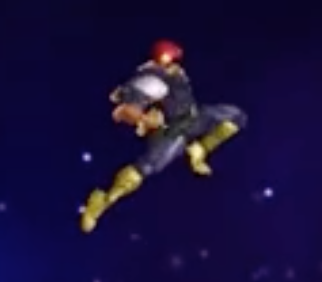
\includegraphics[width=40mm]{logo.png}
	\caption{Agent in action
	\label{overflow}}
\end{figure}

\section{State and Action Space}
The state space is made up of a continuous $(x,y)$ position and a set of discrete parameters describing the state of the agent and its opponent within the game. A few examples of the discrete parameters include the number of remaining lives, if the agent is on the ground, the frame count of the current action, and the animation number. Since the $(x,y)$ position of the agent is continuous, we had the option to either discretize these variables or use a learning algorithm that does not rely on a discrete state space. Discretizing the position variables would still result in an intractible state space so we decided to use a global approximation Q-learning method.

We formulated the action space as a discrete set of controller inputs. This can be adjusted based on the desired complexity of possible actions. For this case we made the action space 54 possible actions and selected the possible controller combinations so that they were meaningful. For example, there exist several combinations of controller inputs that lead to the same action in the game so we decided to trim these non-unique inputs so that the controller inputs in our action space map to a unique action in the game. We decided to discretize the analog stick inputs to three possible values in both the x direction (left, center, and right) and the y direction (down, center, up) as well as allowing only a single button to be pressed at one time (A, B, X, Z, L, or none). This allows us to have a deterministic state evolution based on the given controller input.
\section{Progress}
In order to verify our ideas, we decided to initially train an agent to jump. To do this, we first gathered data from a completely random agent playing the game for 20 minutes. We then constructed what we believed were adequate basis functions, consisting of the agents current height off the ground taken to various powers $\beta(s) = [y, y^2, 1/y]$. The weights $\theta_a$ for different actions for the basis functions were trained using batch-learning global approximation as in algorithm 5.5 of DMU\cite{DMU}. Rewards were assigned when the agent transitioned from being on the ground in state $s_t$ to off the ground in state $s_{t+1}$, and gave penalties when the agent remained on the ground between states $s_t$ and $s_{t+1}$. This initial attempt failed, resulting in an agent that would simply crouch, indicating there were flaws in our strategy required refinement.

First, the initial design resulted in the agent acting every gamestep, inputting 60 actions a second. This is both unrealistic in that the game is not intended to be played with this many inputs, as well as harmful in that it does not allow for state-evolution between action inputs so the bot cannot determine the impacts of a single action on the change in state. The agent was changed so that it now acts on every twelfth frame, corresponding to five times a second. This is a large improvement in that it both better simulates actual gameplay, as well as accommodates the evolution of the state between decisions. It is also beneficial for training as the impacts of a single action are much clearer.

Another flaw to be addressed was the impact of "action-lockout", in which an action taken by the bot may have no impact on its current in game movements due to previous actions taken. An example of this is when the bot inputs a move that has a long wind-up animation that cannot be canceled by other actions. To address this, we now skip over actions input during an "action-lockout" when training the weights of our basis functions so that weights of actions that did not impact the state evolution do not change.

We also believe our initial data set was far too small to train our weights, and decided to regather data. We allowed a random agent to play overnight, gathering 9.5 hours (171,000 samples) worth of data.

Lastly, the basis functions were reworked. Now the basis function $\beta(s)$ is a flag of 0 or 1 for if the agent is on the ground, as well as 400 flags indicating the current action of the agent (i.e. if the agent is currently in animation 326, the 326th element of the basis function for the animations will be a 1 with all the rest being a 0).

The result of these modifications is an agent that has successfully learned to jump. While playing, the agent uses a soft-max strategy to determine which move to select in order to provide some aspect of exploration: $P(a_i) \sim exp(\lambda\beta(s)\theta_a^T)$. Below is a table of the parameters used to train the basis function weights from the random agent data set, as well as the parameters used to play. 

\begin{table}[ht]
\caption{Jumping Agent Training Parameters} 
\centering 
\begin{tabular}{ c | c | c } 
\hline
Parameter & Meaning & Value \\
\hline % inserts single horizontal line
$\alpha$  & Learning Rate & .001\\
$\gamma$ & Future Reward Discount Factor & .95\\
$\lambda$ & Softmax parameter & .1 \\
\hline 
\end{tabular}
\end{table}

While we have to way to quantitativley evaluate the success of the jumping agent, visual inspection shows that the agent has learned to jump as desired.  A video of the agent playing can be viewed here:  \url{https://www.youtube.com/watch?v=ofujaap4MfU}. Our work to date can be viewed on our GitHub repo.

\section{Future Plans}

Future work on this agent will be to give it basis functions as well as rewards corresponding to its distance from the center of the stage in order to penalize the behavior of jumping off the side. From there, we plan on improving our learning process so that the information from each match is processed and the weights on the basis functions are updated before the next match begins, providing a "psuedo" online learning method. We are currently unable to perform true live updates to the weights due computational cost and necessity of having the next action ready in a short time frame. After this, we plan on extrapolating these basis function and creating a new reward function that will allow the agent to learn to fight its opponent. 

\vspace{2mm}

\begin{comment}

%% State Space
\section{State Space}
Our state state space contains the following parameters 

\vspace{2mm}

Non-binary:
\begin{itemize}
\item $x_{a}$ - position of our agent
\item $y_{a}$ - position of our agent
\item $\dot{x}_{a}$ - velocity of our agent
\item $\dot{y}_{a}$ - velocity of our agent
\item $x_{d}$ - distance from our agent to opponent 
\item $y_{d}$ - distance from our agent to opponent 
\item $\dot{x}_{d}$ - relative velocity from our agent to opponent
\item $\dot{y}_{d}$ - relative velocity from our agent to opponent
\end{itemize}

\vspace{2mm}

Binary:
\begin{itemize}
\item $\Upsilon_{1}$ - 1 if not off stage
\item $\Upsilon_{2}$ - 1 if agent has remaining jump
\item $\Upsilon_{3}$ - 1 if agent is facing the opponent
\item $\Upsilon_{4}$ - 1 if the agent in in an attacking state
\item $\Upsilon_{5}$ - 1 if the agent in in an blocking state
\item $\Upsilon_{6}$ - 1 if the opponent in in an attacking state
\item $\Upsilon_{7}$ - 1 if the opponent in in an blocking state
\end{itemize}


\section{Action Space}
Our Action space contains the following parameters to form a reduced set of possible inputs from a gamecube controller. We discretize the analog stick (used to control the movement of agent) and remove redundant inputs.  

\vspace{2mm}

Non-binary:

\begin{itemize}
\item $\Psi_{1}$ - x position of the analog stick
\item $\Psi_{2}$ - y position of the analog stick
\end{itemize}

\vspace{2mm}

Binary:

\begin{itemize}
\item $\Omega_{1}$ - L 
\item $\Omega_{2}$ - B
\item $\Omega_{3}$ - A
\item $\Omega_{4}$ - X
\end{itemize}
\end{comment}

\begin{thebibliography}{999}
\bibitem{DMU}
	Kochenderfer, Mykel,
	\emph{Decision Making Under Uncertainty}.
	The MIT Press, 2015.

\end{thebibliography}


\end{document}

